\chapter{OpenShift}
Im Folgenden werden die Open Source Container Application Platform OpenShift und die dazugehörigen Komponenten beschrieben. OpenShift setzt auf Kubernetes auf. Deshalb wird zuerst Kubernetes in diesem Kapitel erklärt.

\section{Kubernetes}
Container bieten eine Vielzahl an Vorteilen bezüglich der Deploymentzeit, Skalierbarkeit und Größe gegenüber Virtualisierung. Container allein reichen jedoch nicht aus beim Managen von komplexen Cloud Systemen. Es ist sehr einfach, ein paar wenige Container zu starten oder zu stoppen. Wächst die Zahl an Containern, wird das manuelle Management sehr umständlich und aufwändig. \textbf{Container Orchestration Engines (COE)} helfen beim Management vieler Container. COE's bieten Mechanismen zum schnellen Deployen, Zerstören und Skalieren von vielen Containern. Es gibt mehrere Container Management-Lösungen. Die beiden bekanntesten sind Kubernetes und Docker Swarm. Da OpenShift auf Kubernetes aufbaut, wird in diesem Kapitel lediglich Kubernetes behandelt. \cite{LearnOpenShift}.

Grundsätzlich gibt es in Kubernetes zwei verschiedene Arten von Nodes. Wie in Abbildung \ref{fig:KubernetesArchitektur} zu sehen, sind dies der Kubernetes Master und mehrere Kubernetes Nodes.

\subsection{Kubernetes Master}
Der Master-Node ist für das Cluster-Management, die Netzwerk-Allokierung, die Synchronisation und die Kommunikation verantwortlich. Master-Nodes agieren als Hauptansprechspartner für die Clients. Im einfachsten Setup gibt es lediglich einen Master-Node. Hochverfügbare Cluster benötigen aber mindestens zwei Master-Nodes, um häufige Fehlersituationen zu vermeiden. Das wichtigste Service, das am Master läuft, ist die API \cite{LearnOpenShift}.

\subsection{Kubernetes Nodes}
Nodes erledigen die eigentliche Arbeit beim Hosten von Docker Containern. Nodes bieten dabei ein Runtime Environment, in dem die Pods laufen. Auch das Kubelet-Service, das die Pods managt, läuft auf den Nodes.

\begin{figure}[H]
	\begin{center}
		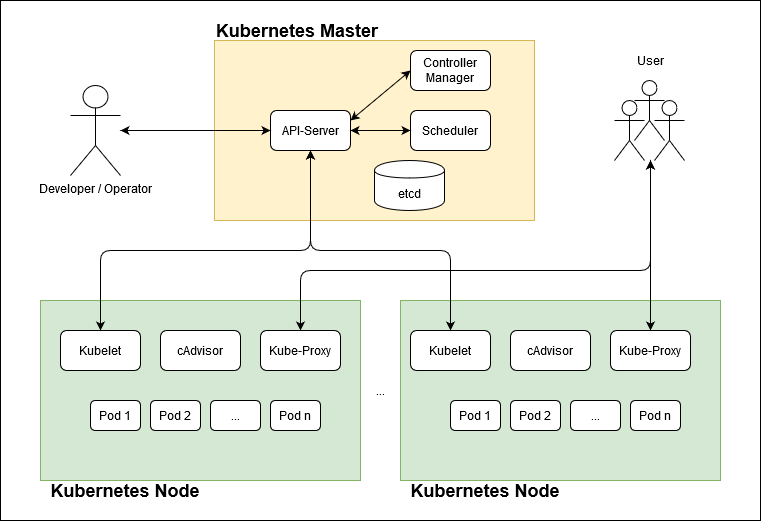
\includegraphics[scale=0.50]{Kubernetes.png}
		\caption[Kubernetes Architektur]{Kubernetes-Architektur \cite{LearnOpenShift}}
		\label{fig:KubernetesArchitektur}
	\end{center}
\end{figure}

\subsection{Kubernetes API}
Die Kubernetes API bietet eine Vielzahl an Ressourcen, um Mechanismen von Kubernetes zu nutzen. Diese Ressourcen können in Form von YAML- oder JSON-Dateien definiert werden. Im Folgenden werden die wichtigsten Ressourcen beschrieben \cite{LearnOpenShift}:

\begin{itemize}
	\item \textbf{Namespaces}: Namespaces dienen zur Separierung von verschiedenen Projekten in der Kubernetes-Umgebung. Sie dienen auch zur Definition von fein granularen Zugriffsrechten. Alle Kubernetes Ressourcen, außer Volumes und Namespaces selbst, leben in einem Namespace. Das heißt, dass deren Name im gegebenen Namespace eindeutig sein muss.
	\item \textbf{Pods}: Pods repräsentieren eine Sammlung von Containern. Jeder Pod ist für eine bestimmte Management Unit in Kubernetes zuständig. Alle Container in einem Pod teilen sich denselben Speicher, dieselben Volumes und dasselbe Netzwerk.
	\item \textbf{Services}: Services repräsentieren ein Interface zwischen Clients und der eigentlichen Applikation, die auf den Pods läuft. Ein Service ist ein Paar aus IP-Adresse und Port, das Netzwerkverkehr zu den Backend Pods im Round-Robin-Verfahren weiterleitet. Dadurch dass Services ein konsistentes Paar aus IP-Adresse und Port sind, werden Clients vor vorübergehenden Änderungen im Cluster geschützt.
	\item \textbf{Replication Controller}: Replication Controller definieren, wie viele Pods repliziert werden müssen. Die Definition von Replication Controller inkludiert Pod Templates, welche die Pods beschreiben. Ein Parameter der Replication Controller ist, wie viele Pods mindestens aufrecht erhalten werden müssen. Stirbt ein Pod, fährt Kubernetes wieder einen hoch, sodass das Minimum erreicht ist.
	\item \textbf{Persistent Volumes}: Persistent Volumes abstrahieren physische Speichersysteme, wie NFS oder iSCSI. Persistent Volumes werden in der Regel von Cluster-Administratoren erstellt und können durch Persistent Volume Claims Binding Mechanismen in einem Pod gemountet werden.
	\item \textbf{Persistent Volume Claims}: Persistent Volume Claims repräsentieren eine Anfrage auf Speicherressourcen. Pod-Definitionen verwenden Persistent Volume Claims nicht direkt. Pods vertrauen auf das Binding von Persistent Volumes zu Persistent Volume Claims.
	\item \textbf{Secrets}: Secrets werden zu Übertragung von sensitiven Daten, wie Schlüssel, Tokens oder Passwörtern innerhalb von Pods verwendet.
	\item \textbf{Labels}: Labels bieten einen Mechanismus zum Spezifizieren eines Gültigkeitsbereichs von Ressourcen. Services verwenden Labels, um den hereinkommenden Netzwerkverkehr zu den richtigen Pods weiterzuleiten. Werden neue Pods mit demselben Label gestartet, werden sie dynamisch dem Service, welches das Label spezifiziert, zugewiesen.
\end{itemize}

\subsection{Kubernetes Master}
Folgende Services laufen auf dem Kubernetes Master \cite{LearnOpenShift}:
\begin{itemize}
	\item \textbf{etcd}: Der etcd ist ein verteilter Key-Value-Konfigurationsspeicher, der alle Metadaten und Cluster Ressourcen enthält. Zur Wahrung der Integrität, wird empfohlen, immer eine ungerade Anzahl an etcd Nodes, beginnend bei drei bei einem hochverfügbaren Setup, laufen zu lassen.
	\item \textbf{Kube-Apiserver}: Der Kube-Apiserver ist ein Service, das die Kubernetes API nach außen frei gibt. Da dieses Service keinen Zustand benötigt, unterstützt es die horizontale Skalierung in hochverfügbaren Clusterkonfigurationen.
	\item \textbf{Kube-Scheduler}: Der Kube-Scheduler ist eine Komponente, die das Erstellen der neu gestarteten Pods überwacht. Dabei muss auf Hardware-Limitierungen, Lokalitätseigenschaften der Daten und Beziehungsregeln geachtet werden.
	\item \textbf{Kube-Controller-Manager}: Der Kube-Controller-Manager managt die Controller. Manche sind Replication Controller, die eine minimale Anzahl an Pods aufrecht erhalten müssen. Weiters werden auch Node Controller gemanagt. Diese überwachen den Zustand der Nodes. Auch Volume Controller, die für das Binding von Persistent Volumes zu Persistent Volume Claims zuständig sind und Endpoint Controller, die Services und Pods verbinden, werden vom Kube-Controller-Manager gemanagt.
	\item \textbf{Cloud-Controller-Manager}: Der Cloud-Controller-Manager bietet eine Integration zu darunterliegenden Cloud Providern, wie DigitalOcean und Oracle Cloud Infrastructure.
\end{itemize}

\subsection{Kubernetes Nodes}
Folgende Services laufen auf den Kubernetes Nodes \cite{LearnOpenShift}:
\begin{itemize}
	\item \textbf{Kubelet}: Dieses Service verwendet eine Pod-Spezifikation, um seine Pods zu managen und periodische Health Checks durchzuführen.
	\item \textbf{Kubeproxy}: Diese Komponente implementiert eine Service-Abstraktion durch Anbieten von TCP und UDP Forwarding über ein Set von Backend Pods.
	\item \textbf{Container Runtime Environment}: Die Container Runtime lädt Images herunter und startet Container. Kubernetes unterstützt dabei Docker und rkt als Container Runtimes.
\end{itemize}

\section{OpenShift}
OpenShift setzt auf Kubernetes auf. Kubernetes bietet Möglichkeiten für die Orchestrierung von Containern, die Elastizität von Pods, Service-Definitionen und Deployment-Konstrukte, um den Status einer Microservice-basierten Applikation zu beschreiben. Es sind jedoch weitere Komponenten nötig, um eine Platform-as-a-Service Plattform zu managen. Kubernetes bietet zum Beispiel kein software-definiertes Netzwerk (SDN) oder Methoden, um den Netzwerkverkehr zu den laufenden Containern zu verteilen. 
All diese Methoden liefert OpenShift mit. 

Die OpenShift-Plattform wurde im Mai 2011 gestartet. Der Source Code war als Open-Source-Projekt frei zugänglich. Red Hat bietet auch eine Enterprise-Version für Deployments an. Dieser Service heißt OpenShift Online.
OpenShift ist eine Plattform, die Entwicklern beim Deployment von Applikationen zu einem oder mehreren Hosts hilft. Diese können jegliche Art von Applikation sein, sei es eine Web Applikation oder eine Backend Applikation. 

Auch Microservices und Datenbanken können in OpenShift deployt werden. Die einzige Voraussetzung ist, dass diese Applikation in einem Container laufen kann.
OpenShift kann auf jedem System laufen, sei es eine öffentliche oder private Infrastruktur, direkt auf physischer Hardware oder einer virtuellen Maschine.
OpenShift bietet dabei auch eine CLI und eine Web Console zur Interaktion mit OpenShift an \cite{DeployingToOpenShift}.


\subsection{OpenShift Master}
Wie in Abbildung \ref{fig:OpenShiftMaster} zu sehen ist, managt der OpenShift Master die Kubernetes Master im OpenShift Cluster. Der OpenShift Master bietet dabei eine REST API für externe Clients zum Managen des OpenShift Masters an. OpenShift bietet dabei auch Features, die von Kubernetes nicht zur Verfügung gestellt werden. Dazu gehören ein rollen- und gruppenbasiertes Sicherheitsmodell und Controller zum Managen von OpenShift Objekten.

\begin{figure}[H]
	\begin{center}
		\includegraphics[scale=0.55]{OpenShiftMaster.png}
		\caption[OpenShift Master]{OpenShift Master \cite{OpenShiftOnline}}
		\label{fig:OpenShiftMaster}
	\end{center}
\end{figure}

Im Folgenden werden die Kernkonzepte und wichtigsten Objekte von OpenShift erklärt.
\subsection{Container und Images}
\textit{Container} sind die Grundbestandteile von OpenShift. Linux Container sind leichtgewichtige Mechanismen zur Isolierung von Prozessen, sodass Prozesse in der Kommunikation miteinander und bei der Nutzung gemeinsamer Ressourcen eingeschränkt sind. Viele Applikationen können in Containern auf einem Host laufen, ohne dass sie auf die Prozesse, Dateien oder das Netzwerk anderer Container zugreifen können. OpenShift und Kubernetes ermöglichen dabei die Orchestrierung von Docker Containern über Mulit-Host-Umgebungen hinweg \cite{OpenShiftOnline}.

Container in OpenShift basieren auf Docker \textit{Images}. Ein Image ist dabei ein Binary, das alle Anforderungen für das Erstellen und Starten eines Containers, sowie Metadaten, welche Anforderungen der Container beschreiben, beinhaltet.
Container haben nur Zugriff auf Ressourcen, die im Image definiert wurden, außer dem Container werden weitere Rechte für den Zugriff auf Dateien eingeräumt. Beim Deployment eines Image auf mehreren Containern über verschiedene Hosts hinweg kann OpenShift Redundanzen und horizontale Skalierung bieten \cite{OpenShiftOnline}.

\subsection{Pods und Services}
Ein \textit{Pod} ist eine Einheit aus einem oder mehreren Containern auf einem Host und die kleinste Recheneinheit, die definiert, deployt und gemanagt werden kann. Jedem Pod wird eine interne IP-Adresse zugewiesen. Container innerhalb eines Pods können dadurch ihren lokalen Speicher und das Netzwerk teilen.
Pods haben einen Lebenszyklus. Pods werden definiert und danach einem Node zugewiesen. Dann laufen sie solang, bis sie gelöscht oder aus anderen Gründen entfernt werden. Pods können nach dem Stoppen entweder gelöscht oder behalten werden. Dadurch kann auch nach Absturz eines Pods auf die Log-Files zugegriffen werden \cite{OpenShiftOnline}. OpenShift behandelt Pods, als wären sie unveränderbar. Änderungen an laufenden Pods können nicht vorgenommen werden. OpenShift implementiert Änderungen an Pods durch Terminieren des Pods und Starten eines neuen geänderten Pods. Ein Pod  behält dabei nicht seinen Zustand \cite{OpenShiftOnline}.

Ein Kubernetes \textit{Service} dient als interner Load Balancer. Es leitet Verbindungen, die es bekommt, an ein Set von replizierten Pods weiter. Pods können dabei zum Service hinzugefügt und entfernt werden. OpenShift vergibt Default Service Cluster IP-Adressen. Dadurch wird Pods die Kommunikation mit anderen Pods ermöglicht. Um auch externen Zugriff auf die Services zu ermöglichen, können dem Service auch \textit{externalIP}- und \textit{ingressIP}-Adressen zugewiesen werden. Diese externalIP-Adressen können auch virtuelle IP-Adressen sein, die hochverfügbaren Zugriff auf das Service ermöglichen.
Services wird ein Paar aus IP-Adresse und Port zugewiesen. Falls darauf zugegriffen wird, wird die Verbindung auf einen passenden Pod weitergeleitet. Ein Service verwendet dabei einen Label Selector, um alle laufenden Container, die ein spezifisches Netzwerk-Service auf einem spezifischen Port laufen lassen, zu finden \cite{OpenShiftOnline}.

\subsection{User, Namespaces und Projekte}
Die Interaktion mit OpenShift ist mit \textit{Usern} assoziiert. Ein OpenShift \textit{User}-Objekt repräsentiert einen Akteur, dem verschiedene Rechte im System durch das Hinzufügen von Rollen zu den Usern oder deren Gruppen eingeräumt werden \cite{OpenShiftOnline}.
Dabei gibt es grundsätzlich drei verschiedene Arten von User Objekten \cite{OpenShiftOnline}:
\begin{enumerate}
	\item \textbf{Regular User}: Die meisten User in OpenShift gehören zu dieser Gruppe. Regular User werden automatisch beim ersten Login vom System erstellt oder können durch die API selbst erstellt werden. Regular User werden durch das User-Objekt repräsentiert. \linebreak
	Beispiele sind \textit{joe}, \textit{alice}
	\item \textbf{System User}: Viele der System User werden automatisch erstellt, sobald die Infrastruktur definiert wurde, hauptsächlich für die sichere Interaktion mit der API. Dazu gehören ein Cluster-Administrator, der Zugriff auf alle Komponenten hat, ein Per-Node-User und User für die Nutzung von Router und Registries. Es gibt auch einen \textit{anonymous} System User, der bei unautorisierten Requests verwendet wird. \linebreak
	Beispiele sind \textit{system:admin}, \textit{system:openshift-registry}, \textit{system:node:node1.example.com}.
	\item \textbf{Service Accounts}: Service Accounts sind spezielle System User, die mit einem Projekt assoziiert sind. Manche werden beim Erstellen eines Projekts automatisch erstellt. Projektadministratoren können mehr Rechte für den Zugriff auf das Projekt definieren. Service Accounts werden durch das ServiceAccount-Objekt repräsentiert. \linebreak
	Beispiele sind \textit{system:serviceaccount:default:deployer}, \textit{system:serviceaccount:foo:builder}.
\end{enumerate}

Jeder User muss sich vor der Nutzung von OpenShift authentifizieren. API-Requests ohne Authentifizierung oder einer invaliden Authentifizierung werden mit dem \textit{anonymous}-User durchgeführt. Sobald der User authentifiziert ist, definiert eine Policy, welche Aktionen der User durchführen darf \cite{OpenShiftOnline}.

Ein Kubernetes \textit{Namespace} bietet einen Mechanismus zur Isolierung von Ressourcen in einem Cluster. Namespaces bieten einen Isolationsbereich für \cite{OpenShiftOnline}:
\begin{itemize}
	\item benannte Ressourcen, um Namenskollisionen zu vermeiden,
	\item Management Authorities für User,
	\item die Möglichkeit, Ressourcennutzung zu limitieren.
\end{itemize}
Die meisten Objekte im System sind durch Namespaces isoliert. Nodes und User unterliegen jedoch keinem Namespace.

Ein \textit{Projekt} ist ein Kubernetes-Namespace mit zusätzlichen Annotationen. In Projekten wird auch der Zugriff von Usern auf Ressourcen gemanagt. Ein Projekt erlaubt einer Menge von Usern, deren Ressourcen von anderen Usern getrennt zu organisieren und zu managen. User müssen die Rechte für Projekte von Administratoren zugewiesen bekommen, außer ein User erstellt selbst ein Projekt. Dann hat er auf dieses Projekt automatisch Zugriff.
Projekte können separate \textit{Namen}, \textit{Anzeigenamen} und \textit{Beschreibungen} haben.
\begin{itemize}
	\item \textbf{Name}: Der zwingend notwendige Name ist ein eindeutiger Indikator für das Projekt und ist sichtbar bei der Verwendung der CLI Tools oder der API. Die maximale Länge des Namens beträgt 63 Zeichen.
	\item \textbf{Anzeigename}: Der Anzeigename zeigt, wie das Projekt in der Web Console dargestellt wird. Ist dieser Wert nicht vorhanden, wird der eindeutige Name angezeigt.
	\item \textbf{Beschreibung}: Die optionale Beschreibung ist eine detaillierte Beschreibung des Projekts und ist auch in der Web Console sichtbar.
\end{itemize}

Jedes Projekt isoliert ein Set von \cite{OpenShiftOnline}:
\begin{itemize}
	\item \textbf{Objekten}: Pods, Services, Replication Controller, etc,
	\item \textbf{Policies}: Regeln für User zur Interaktion mit Objekten,
	\item \textbf{Constraints}: Teile von Objekten, die limitiert werden können,
	\item \textbf{Service Accounts}: bieten einen flexiblen Weg, um den Zugriff auf die API zu kontrollieren.
\end{itemize}

Cluster-Administratoren können Projekte erstellen und administrative Rechte für Projekte vergeben. Cluster-Administratoren können auch Entwickler das Erstellen von Projekten erlauben. Entwickler und Administratoren können durch die CLI oder die Web Console mit Projekten interagieren.


\subsection{Builds und Image Streams}
Ein \textit{Build} ist der Prozess der Transformation von Input-Parametern in Objekte. Meistens werden Builds zur Transformation von Input-Parametern oder Source Code in ausführbare Images genutzt. Ein BuildConfig-Objekt beschreibt dabei den Build-Prozess \cite{OpenShiftOnline}.

OpenShift bietet dabei erweiterbaren Support für Build-Strategien. Es stehen vier Build-Strategien zur Verfügung \cite{OpenShiftOnline}:
\begin{enumerate}
	\item \textbf{Docker Build}: Die Docker Build-Strategie führt einen Docker Build aus und benötigt dadurch ein Repository mit einem Dockerfile und allen Artifakten, um das Docker Image zu erstellen.
	\item \textbf{Source-to-Image (S2I) Build}: S2I ist ein Tool zum Bauen von reproduzierbaren Docker Containern und Docker Images. Dadurch werden startfähige Docker Images durch Injizieren des Source Code der Applikation erstellt. Das neue Docker Image übernimmt das Basis Image, auch Builder Image genannt, und die gebauten Sourcen. Auf das neue Docker Image kann dann ein \textit{docker run} ausgeführt werden. S2I unterstützt inkrementelle Builds, welche vorher heruntergeladene Abhängigkeiten wiederverwenden.
	\item \textbf{Custom Build}: Die Custom Build-Strategie erlaubt Entwicklern spezifische Builder Images zu definieren. Dadurch können die Build-Prozesse angepasst werden.
	Ein Custom Builder Image ist ein Docker Container Image eingebettet in Build-Prozess-Logik, z.B. zum Erstellen von Basis Images. Als Beispiel für ein Custom Builder Image steht auf der Seite von \href{https://hub.docker.com/}{Docker Hub} (https://hub.docker.com/) das Image \textit{openshift/origin-custom-docker-builder} zur Verfügung.
	\item \textbf{Pipeline Build}: Die Pipeline Build-Strategie erlaubt Entwicklern eine Jenkins Pipeline zu erstellen. Dieser Build kann ebenso wie die anderen Build-Strategien gestartet, gemonitort und gemanagt werden. Pipeline Workflows werden in einem Jenkinsfile - entweder eingebettet in der Build-Konfiguration oder eigens im Git Repository - definiert. Bei der ersten Definition einer Build Konfiguration mit der Pipeline-Strategie instanziert OpenShift einen Jenkins Server, der die Pipeline ausführt. Darauffolgende Pipeline Build-Konfigurationen nutzen diesen Jenkins Server.
\end{enumerate}

\textit{Image Streams} und die dazugehörigen Image Stream Tags bieten eine Abstraktion des Docker Images. Die Image Streams und Image Stream Tags erlauben das Anzeigen der verfügbaren Images und stellen sicher, dass das richtige Image verwendet wird, auch wenn sich das Repository ändert.
Image Streams enthalten keine Image-Daten, repräsentieren aber eine virtuelle Sicht auf die zusammenhängenden Images, ähnlich einem Image Repository \cite{OpenShiftOnline}.

Es können auch Builds und Deployments konfiguriert werden, um Notifizierungen zu bekommen, sobald neue Images hinzugefügt werden.
Wenn zum Beispiel ein Deployment ein spezifisches Image benutzt und eine neue Version dieses Image erstellt wird, kann automatisch ein neues Deployment mit der neuen Version getriggert werden.
Solange der Image Stream Tag nicht upgedatet wird, benutzt das Deployment dieselbe Version des Image, auch wenn eine neue Version verfügbar wäre \cite{OpenShiftOnline}.

\subsection{Replication Controller, Jobs und Deployments}
\textit{Replication Controller} stellen sicher, dass eine in der Konfiguration spezifizierte Anzahl an Replikas eines Pods immer laufen. Falls ein Pod abstürzt oder gelöscht wird, instanziert der Replication Controller so viele Replikas, bis das Minimum wieder erreicht ist \cite{OpenShiftOnline}.
Die Konfiguration eines Replication Controllers besteht aus \cite{OpenShiftOnline}:
\begin{itemize}
	\item der gewünschten Anzahl an Replikas (dieser Wert kann auch zur Laufzeit geändert werden),
	\item einer Pod Definition zum Erstellen eines Pods,
	\item einem Selector zum Identifizieren der gemanagten Pods.
\end{itemize}
Ein Selector ist dabei ein Set von Labels, die einem Pod zugewiesen werden. Die Labels sind in der Pod Definition enthalten. Durch die Selectors bestimmt der Replication Controller die Anzahl an Pods, die gerade laufen und fügt bei Bedarf neue hinzu oder löscht welche.
Der Replication Controller übernimmt nicht die Autoskalierung basierend auf der Load oder dem Traffic. Dazu muss ein externer Auto-Scaler definiert werden \cite{OpenShiftOnline}.

Ein \textit{Job} verhält sich ähnlich zu einem Replication Controller. Auch ein Job erstellt Pods für spezielle Zwecke. Der Unterschied zum Replication Controller ist, dass Replication Controller für Pods designt sind, die durchgehend laufen und Jobs lediglich für Pods zuständig sind, die einen gewissen Arbeitsauftrag erledigen und danach wieder herunterfahren. Der Job überwacht die erfolgreichen Fertigstellungen und fährt herunter, sobald alle von ihm überwachten Pods erfolgreich fertiggestellt sind.

OpenShift bietet durch \textit{Deployments} und Deployment Configurations erweiterten Support für die Softwareentwicklung und den Deployment Lifecycle. Im einfachsten Fall erstellt ein Deployment lediglich einen neuen Replication Controller und lässt diesen Pods starten. Deployments bieten auch die Möglichkeit aus bestehenden Deployments und Images neue Deployments zu erstellen. Auch Hooks, die vor oder nach dem Erstellen eines Replication Controllers laufen, können definiert werden \cite{OpenShiftOnline}.
Ein DeploymentConfig-Objekt definiert dabei folgende Details \cite{OpenShiftOnline}:
\begin{itemize}
	\item die Definition eines Replication Controllers,
	\item Trigger, um neue Deployments automatisch zu erstellen,
	\item eine Strategie zum Wechseln zwischen Deployments,
	\item Life-Cycle-Hooks.
\end{itemize}
Jedes Mal wenn ein Deployment getriggert wird, egal ob automatisch oder manuell, managt ein Deployer Pod das Deployment. Dazu gehören auch das Herunterskalieren des alten Replication Controllers, das Hochskalieren des neuen Replication Controllers und das Ausführen der Hooks.
Der Deployment Pod bleibt nach Fertigstellung auf unbestimmte Zeit am Leben, um die Logs des Deployments aufrufen zu können \cite{OpenShiftOnline}. 

\subsection{Routes}
OpenShift gibt einen Service durch \textit{Routes} nach außen frei, sodass externe Clients ihn erreichen können. DNS-Auflösung für den Hostnamen wird separat übernommen. Jede Route besteht aus einem Namen, limitiert auf 63 Zeichen, einem Selector und einer optionalen Sicherheitskonfiguration.
Administratoren können Router zu Nodes deployen. Dadurch können externe Clients die Routen, die von Entwicklern erstellt wurden, aufrufen. Ein Router benutzt dabei einen Service Selector, um die Services und die Endpoints zu finden. Wenn Router und Service Load Balancing erlauben, wird das Load Balancing automatisch eingerichtet \cite{OpenShiftOnline}.

\subsection{Templates}
\textit{Templates} beschreiben ein Set von Objekten, die parametriert und prozessiert werden können, um eine Liste von Objekten zu erstellen. Ein Template kann jedes Objekt, zu dessen Erstellung der User die Rechte besitzt, beschreiben. Dazu gehören Services, Build-Konfigurationen und auch Deployment-Konfigurationen. Ein Template kann auch ein Set von Labels definieren, die dann auf die erzeugten Objekte angewandt werden.
Eine Liste von Objekten durch ein Template kann über die CLI oder die Web Console erstellt werden \cite{OpenShiftOnline}. 
